%!TEX root = ../main.tex

\chapter{Preliminary project}
\noindent
The project is made by three main components: \ac{VR} APP, backend, webui. This chapter will talk about them.
\section{The VR APP}
\noindent
This section will explain the main choices behind the \ac{VR} APP
\paragraph{The development environment:} 
There are three main way to develop on the Meta Quest 2:

\begin{itemize}
  \item \textbf{Native:} By using native \ac{API} that Meta provides for the \ac{HMD}.
  \item \textbf{Unity:} Is a famous game engine principally used for lightweight video games, It is pretty functional and easy to use, its programming language is \verb|C#|. 
  \item \textbf{Unreal Engine:} Is a famous game engine used for big games, its performance is the best in the market, it uses \cpp and a graphical programming language called Blueprint. 
\end{itemize}
\noindent
As we said in the non-functional requirements we will use a game engine, I have opted for \ac{UE} because of its performance, the 3D models are pretty complex (\textasciitilde10MByte in size),
so we need good performance.
It has a lot of tools for multiplayer and a nice documentation other than a big community of developers.

\section{Unreal Engine}
\noindent
Made by Epic Games, the project was born for the video game Unreal, now is one of the best engine that power a lot of important video games and 3D animation.
For this project it will be used the 5.2.1 version for the best compatibility with the \ac{HMD}, still is not an old version, the last one is 5.3. 

\paragraph{The fundamentals:}
\ac{UE} has a 3D preview mode that let the user set the various 3D objects in the scene. 
In unreal a scene is called "Level", each element in a level is called "Actor", Actors are made by multiple components.\\
Each element of unreal can be build with a propriety system called Blueprint, a visual programming interface, or via \cpp, or by combine them.
Principally Blueprint can make the developing of the project faster and easier at the cost of performance, \cpp perform better, and it has a bigger range of tools.
So It is important to combine both languages for having the best performance and flexibility in the project.\\
Like a lot of game engines, \ac{UE} tries to render as much frame as much as possible, each cycle of rendering is called tick.\\
Its important that long actions must be asynchronous respect the game ticks, and if something must be runner in the so-called "game thread", it must be as fast as possible so that the frame rate does not drop to a certain level.

\paragraph{Events:}
Events are what start the execution of code inside a Blueprint. Each blueprint have its own standard event, they depend on the object, the basic ones are:
\begin{itemize}
  \item \textbf{Begin Play:} runs one time when the actor is spawned (this is not a constructor).
  \item \textbf{On tick:} runs on every game tick.
\end{itemize}
\noindent
But we can also create custom event with Blueprint or \cpp, they can be triggered whenever we want, they can also be replicated in clients in multiplayer sessions. 
Like functions, events can have inputs but not outputs.

\paragraph*{Multiplayer:}
\ac{UE} just support a client-server configuration for manage multiplayer session, it has two main implementation: Stand-Alone server and listening server.\\
Stand-Alone server consist in having a server that emulates the gaming session, it requires a server powerful enough to run the basic function of the game event if it does not need to render it.\\
Listening Server does not need a Stand-Alone server, simply one device acts not only as a client but also as a server. Normally client-server is the best in performance and latency, but because this software is simple, the listening server is the right implementation.

\section{Network Infrastructure}
\noindent
The Network Infrastructure [fig:\ref{fig:NetworkSchema}] it is simple, a server will be hosted in the IT department of the hospital that will host the \ac{REST} server for managing 3D Models and multiplayer sessions,
and in the same server will host via NODEjs the Web Portal for managing the 3DModels.
The multiplayer itself will be manage by the host \ac{HMD}

\begin{figure}[h]
  \centering
  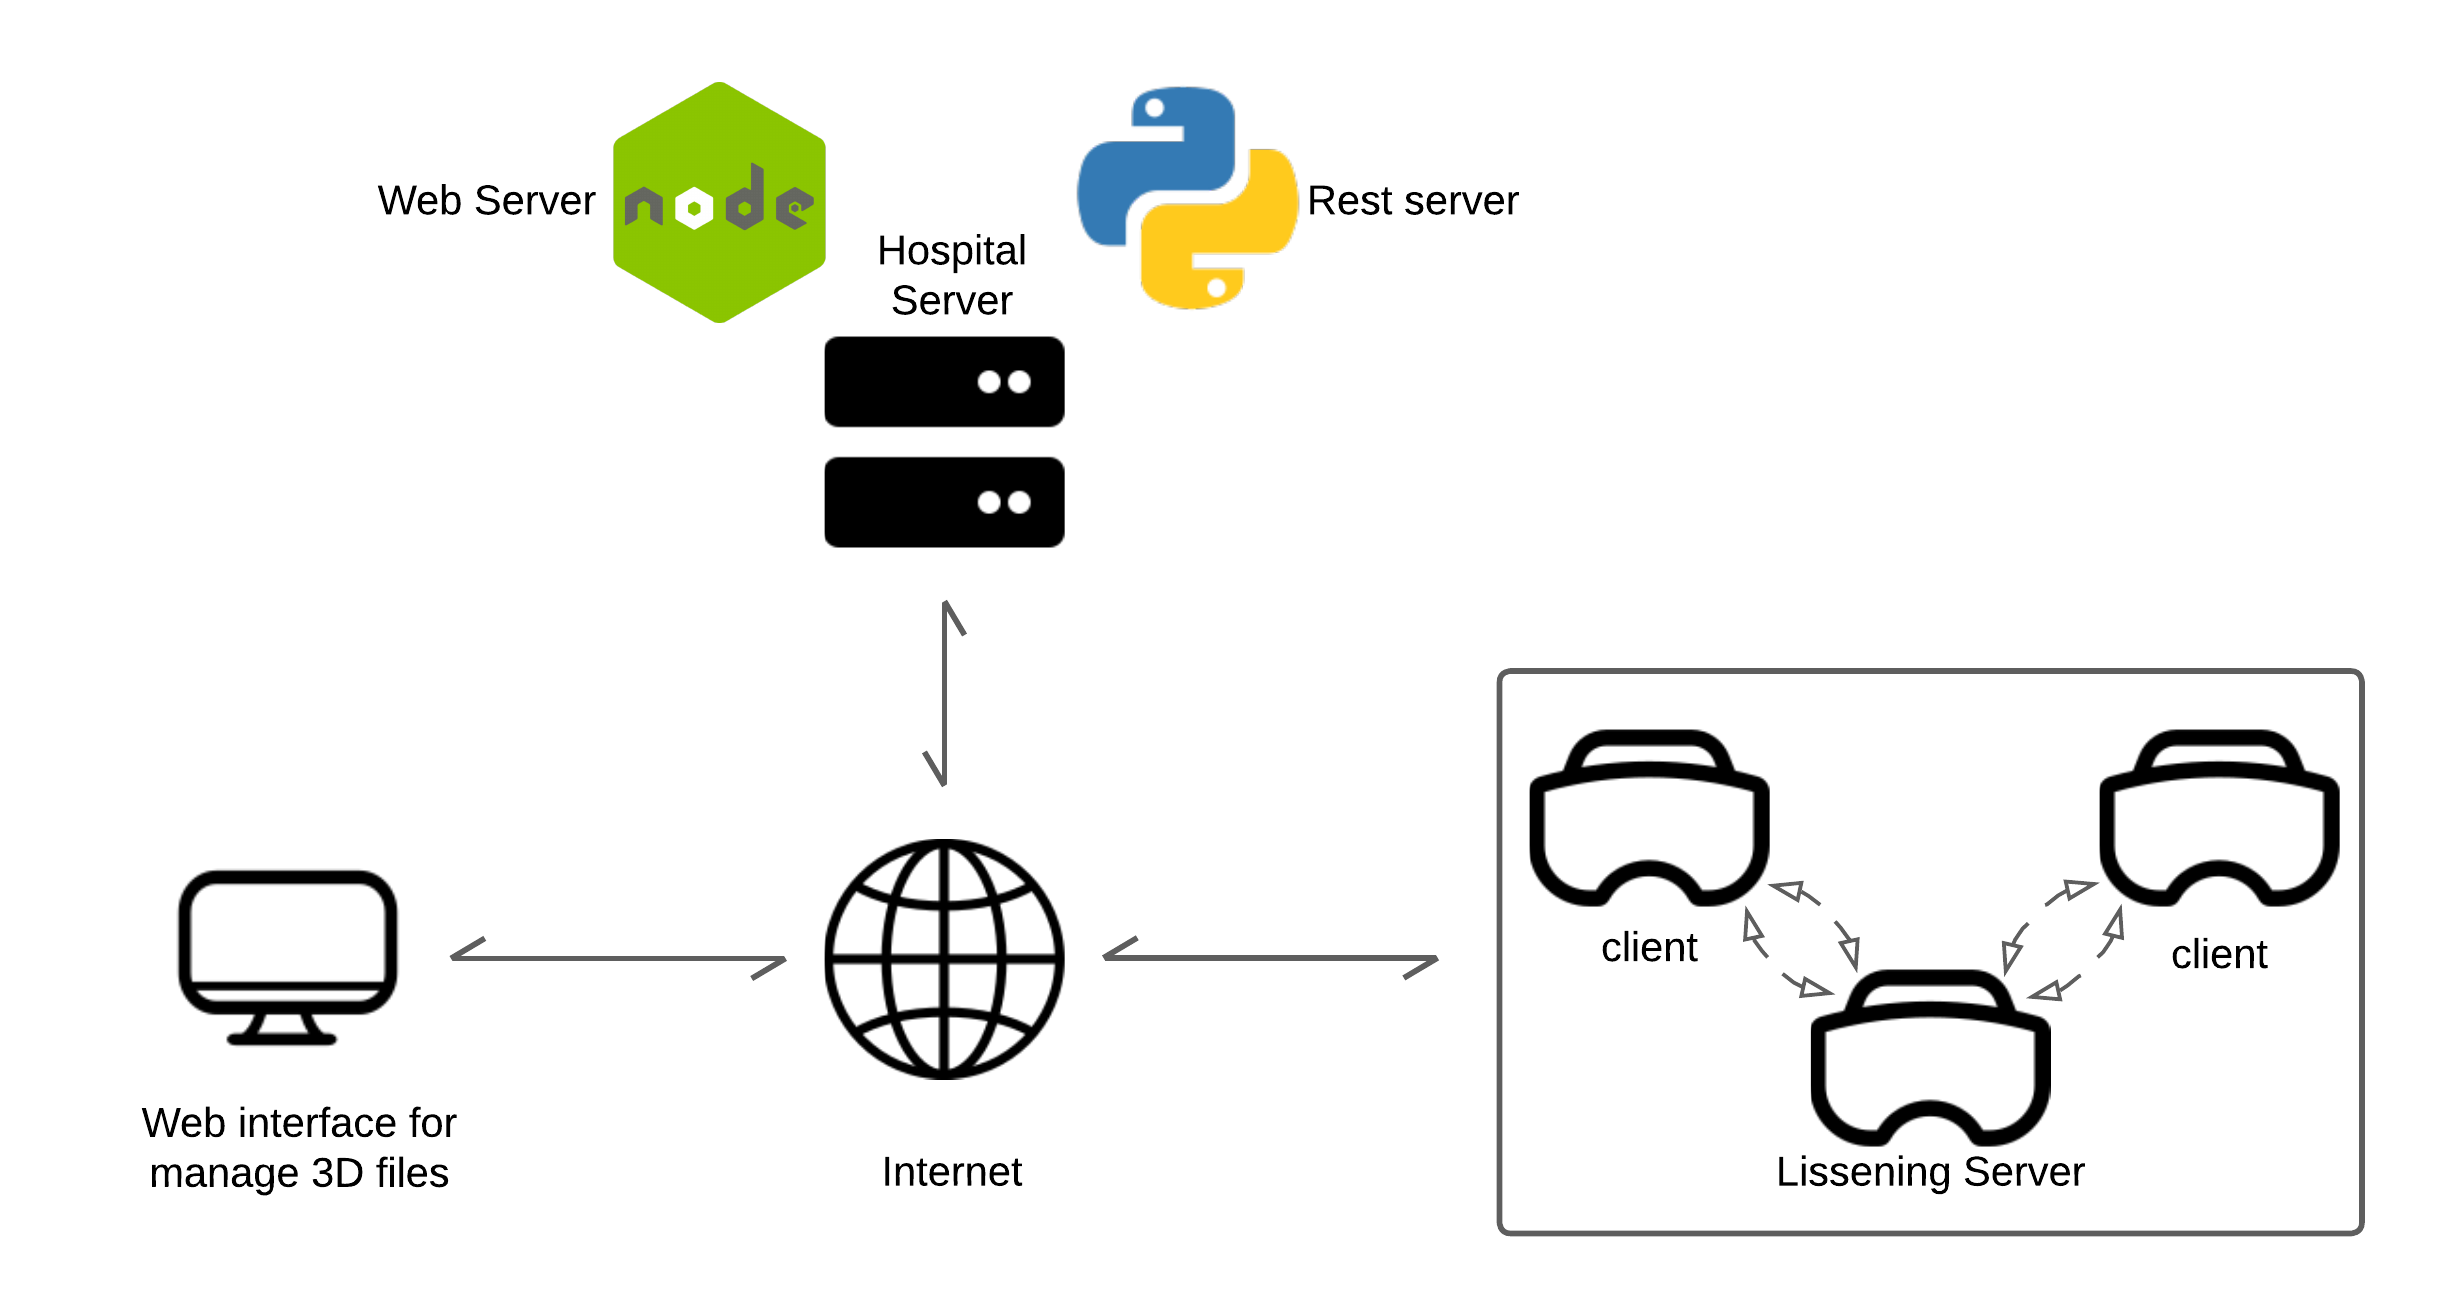
\includegraphics[width=\textwidth]{networkSchema.png}
  \caption{Network Schema}
  \label{fig:NetworkSchema}
\end{figure}


\paragraph{The backend:}
The backend is a simple Python program that it functions as a \ac{REST} server, were each 3D model is a resource.
It also manages the multiplayer session by creating the session code, and save the \ac{IP} address of the listening server.
The library used is called Flask\footnote{\url{https://flask.palletsprojects.com/en/3.0.x/}}, it simply let you run a function respect to a \ac{HTTP} response received.

\paragraph{The WebUI}
The WebUI is made with reactJS, a popular framework for website, the main reason of this choice is for faster development because its community is massive, in fact will be using a UI library called MUI\footnote{\url{https://mui.com/}}
and a 3D library for rendering 3D models called React Three Fiber\footnote{\url{https://r3f.docs.pmnd.rs/getting-started/introduction}}.\\
The main functionality of the WebUI will be:
\begin{itemize}
  \item previewing 3D models with the right colors 
  \item upload 3D models
  \item delete 3D models
\end{itemize}



